\clearpage

\section {Oscillation fitting method} 
\label{sec:fitting}

\subsection {Outline}

Measurements of the oscillation parameters $sin^{2}2\theta_{23}$, $\Delta m^{2}_{23}$
are obtained by comparing the observed and predicted SuperK reconstructed energy spectra
for 1-ring $\mu$-like events.
Let $N$ be the number of reconstructed energy bins and
${\bf a}$ be a $1 \times N_{s}$ - dimensional array of systematic (nuisance) 
parameters that affect the SuperK reconstructed energy spectrum prediction (e.g
parameters that control the beam and neutrino interaction simulations and 
the detector response).
Best-fit values are obtained by minimizing: 
\begin{equation}
\displaystyle
\chi^{2} (sin^{2}2\theta_{23},\Delta m^{2}_{23}; {\bf a}) = 
  2 \cdot \sum_{i=0}^{N-1} 
   \Big( 
     n^{obs}_{i} \cdot ln(n^{obs}_{i}/n^{exp}_{i}) +
     (n^{exp}_{i}-n^{obs}_{i}) 
   \Big) +
   ({\bf a}-{\bf a_{0}})^{T} \cdot {\bf C}^{-1} \cdot ({\bf a}-{\bf a_{0}})
\label{eq:chisquare}
\end{equation}
where
${\bf a_{0}}$ is an $1 \times N_{s}$ - dimensional array with the default values of 
considered systematics parameters, ${\bf a}^{T}$ is the transpose of ${\bf a}$,
${\bf C}$ is the systematic parameter covariance matrix of dimension $N_{s} \times N_{s}$,
$n^{obs}_{i}$ is the observed number of events in the $i^{th}$ bin, and
$n^{exp}_{i} = n^{exp}_{i}(sin^{2}2\theta_{23},\Delta m^{2}_{23}; {\bf a})$ 
is the corresponding expected number of events.

Due to the limited statistics in SuperK 
and the limited amount of information available to this analysis from the near detectors,
we do not fit for systematics.  Instead, we evaluate oscillation systematics as described
in section \ref{sec:eval_osc_systematics}.



%
%
% Likelihood function & 
% Comparison of K2K/MINOS fit methods
%
%

\subsection {Construction of the likelihood function and comparison of the `MINOS' and `K2K' methods }
\label{sec:K2K_MINOS_fit_comparison}

In this analys, we use a fitting method previously employed by MINOS \cite{MinosDisappearanceAnalysis}.
The construction of the likelihood function is described in this section in detail.
We use a likelihood ratio method, 
whereas J.Kameda's analysis uses a
%%\footnote
%%{ 
%%  Input p.d.f's come from Monte Carlo samples that have an intrinsic 50 MeV energy binning 
%%  (binning of the flux histograms used during event generation).
%%}
maximum likelihood
method previously employed by K2K \cite{K2KDisappearanceAnalysis}.
These two methods give identical results for the best-fit oscillation parameters (for same input p.d.f's).

Let ${\bf n^{obs}}$ be a set of $N$ measurements (the number of events in each of the $N$ bins
\footnote
{
  In this analysis we use 200 50-MeV bins in the 0-10 GeV reconstructed neutrino energy range.
}
).
The probability density function (p.d.f.) for the total number of events 
$n^{obs}_{tot} = \sum_{i=0}^{N-1} n^{obs}_{i}$
observed in SuperK has a 
Poisson distribution, and the mean of that distribution is equal to the predicted total number 
of events $n^{exp}_{tot} = n^{exp}_{tot}(sin^{2}2\theta_{23},\Delta m^{2}_{23}; {\bf a})
= \sum_{i=0}^{N-1} n^{exp}_{i}(sin^{2}2\theta_{23},\Delta m^{2}_{23}; {\bf a})$. 
The p.d.f. is
\begin{equation}
\begin{array}{rcl}
\displaystyle
f_{poisson} = 
f_{poisson}({\bf n^{obs}}; sin^{2}2\theta_{23},\Delta m^{2}_{23}; {\bf a}) = 
   \frac{\left[n^{exp}_{tot}\right]^{n^{obs}_{tot}}
   e^{-n^{exp}_{tot}}}{n^{obs}_{tot}!} 
\end{array}
\label{eq:pdf_poisson}
\end{equation}

The reconstructed energies of the observed events are distributed over $N$ bins. 
Since there are $N$ possible outcomes for the process of placing an event in a bin, 
the p.d.f.\ of the distribution of those outcomes is multinomial:
\begin{equation}
\begin{array}{rcl}
\displaystyle
f_{multinomial} = 
f_{multinomial}({\bf n^{obs}}; sin^{2}2\theta_{23},\Delta m^{2}_{23}; {\bf a}) = 
   n^{obs}_{tot}!\prod_{i=0}^{N-1} 
   \frac{1}{n^{obs}_{i}!} 
   P_{i}^{n^{obs}_{i}} 
\end{array}
\label{eq:pdf_multinomial_1}
\end{equation}
where $P_{i} = P_{i}(sin^{2}2\theta_{23},\Delta m^{2}_{23}; {\bf a})$
is the probability that an event is placed in the $i^{th}$ bin. 
This probability can be calculated as the ratio of the 
number of events predicted for that bin to the predicted total number of events:
\begin{equation}
\displaystyle
  P_{i} = 
  \frac{n^{exp}_{i}(sin^{2}2\theta_{23},\Delta m^{2}_{23}; {\bf a})}
       {n^{exp}_{tot}(sin^{2}2\theta_{23},\Delta m^{2}_{23}; {\bf a})}
\label{eq:prob_in_multinomial}
\end{equation}
Therefore, $f_{multinomial}$ can be written as
\begin{equation}
\begin{array}{rcl}
\displaystyle
f_{multinomial} = 
   n^{obs}_{tot}!\prod_{i=0}^{N-1} \frac{1}{n^{obs}_{i}!} 
   \left[\frac{n^{exp}_{i}}
              {n^{exp}_{tot}} \right]^{n^{obs}_{i}} 
\end{array}
\label{eq:pdf_multinomial_2}
\end{equation}

The joint p.d.f.\ $f_{joint} = f({\bf n^{obs}}; sin^{2}2\theta_{23},\Delta m^{2}_{23}; {\bf a})$ 
for the outcome of the reconstructed energy distribution 
is the product of the Poisson and multinomial distributions
shown in Eq.\ \ref{eq:pdf_poisson} and Eq.\ \ref{eq:pdf_multinomial_2} 
respectively:
\begin{equation}
\displaystyle
f_{joint} = 
   e^{-n^{exp}_{tot}} 
   \prod_{i=0}^{N-1} \frac{1}{n^{obs}_{i}!} 
   \left[n^{exp}_{i}\right]^{n^{obs}_{i}} 
\label{eq:reco_hist_pdf}
\end{equation}
 
In our analysis, we use the p.d.f.\ in Eq.\ \ref{eq:reco_hist_pdf}, and this is identical to the likelihood function used 
by K2K in \cite{K2KDisappearanceAnalysis}: 
L$_{NORM}$ corresponds to the Poisson term and L$_{SHAPE}$ to the multinomial term. 
However there is also a difference between the two analyses. K2K used the ``maximum likelihood'' method, i.e.\ the best-fit 
values of the oscillation parameters were obtained by taking the natural 
logarithm of Eq.\ \ref{eq:reco_hist_pdf}, and maximising it with respect to those parameters. We use the ``likelihood ratio''
method, which involves dividing the p.d.f. in Eq.\ \ref{eq:reco_hist_pdf} by a factor that does not depend on the oscillation parameters.
The best-fit values of the oscillation parameters are unchanged by such a division (see \cite{StatAnalysisCowan} for 
further details). 

In our analysis, the p.d.f.\ in Eq.\ \ref{eq:reco_hist_pdf} is divided by

\begin{equation}
\displaystyle
f_{0} = f_{0}({\bf n^{obs}}) = 
  \frac{\left[n^{obs}_{tot}\right]^{n^{obs}_{tot}}e^{-n^{obs}_{tot}}}{n^{obs}_{tot}!} n^{obs}_{tot}! 
       \prod_{i=0}^{N-1} \frac{1}{n^{obs}_{i}!} \left[\frac{n^{obs}_{i}}{n^{obs}_{tot}} \right]^{n^{obs}_{i}}
\label{eq:division_factor}
\end{equation}
Cancelling the factors of $n^{obs}_{tot}!$ and using $n^{obs}_{tot} = \sum_{i=0}^{N-1}n^{obs}_{i}$, Eq.\ \ref{eq:division_factor} simplifies to
\begin{equation}
\displaystyle
f_{0} = 
  e^{-n^{obs}_{tot}}  
  \prod_{i=0}^{N-1} 
  \frac{1}{n^{obs}_{i}!} \left[n^{obs}_{i} \right]^{n^{obs}_{i}}
\label{eq:division_factor_simple}
\end{equation}
Dividing Eq. \ref{eq:reco_hist_pdf} by Eq. \ref{eq:division_factor_simple} gives the likelihood ratio $\lambda$:
\begin{equation}
\displaystyle
\lambda = e^{n^{obs}_{tot}-n^{exp}_{tot}} 
   \prod_{i=0}^{N-1} \left(\frac{n^{exp}_{i}}{n^{obs}_{i}} \right)^{n^{obs}_{i}}
\label{eq:lambda}
\end{equation}
In the large-sample limit, the quantity
\begin{equation}
\displaystyle
-2 \, \textrm{ln} \lambda = 
   2 \sum_{i=0}^{N-1} 
   \left[n^{obs}_{i} \: \textrm{ln} \left(\frac{n^{obs}_{i}}{n^{exp}_{i}} \right) + 
   n^{exp}_{i} - n^{obs}_{i} \right]
\label{eq:minusloglambda}
\end{equation}
has a $\chi^{2}$ distribution. Best-fit values of the oscillation parameters 
are obtained by varying their values in the input to
$n^{exp}_{i}$ until the minimum of -2ln$\lambda$ is found. 
The reader should compare Eq. \ref{eq:minusloglambda} with the statistical
term of Eq. \ref{eq:chisquare} shown in previous section.


\subsection {Oscillation parameter range}
\label{sec:osc_par_limits}

The search for the minimum value of 
$\chi^{2} (sin^{2}2\theta_{23},\Delta m^{2}_{23}; {\bf a})$ (see Eq. \ref{eq:chisquare}) 
is performed in the range 
$0 \leq$ $sin^{2}2\theta_{23}$ $\leq 1$ and
$1 \times 10^{-3} eV^{2}/c^{4} \leq$ $|\Delta m^{2}_{23}|$ $\leq 6 \times 10^{-3} eV^{2}/c^{4}$.
Values of $sin^{2}2\theta_{23}$ $> 1$  are not permitted; although it is numerically allowed and,
occasionally, it yields better fits to data, it has no physical interpretation within the context
in which we attempt to interpret the data (2-flavour neutrino oscillations) and causes p.d.f's to 
have pathological behaviour.
The maximum allowed value of $|\Delta m^{2}_{23}|$ is $6 \times 10^{-3} eV^{2}/c^{4}$.
Due to the sinusoidal nature of the oscillation survival probability function,
statistical fluctuations in the present small-statistics dataset can, very rarely, 
cause a global minimum in large $|\Delta m^{2}_{23}|$ ($> 6 \times 10^{-3} eV^{2}/c^{4}$). 
As a $|\Delta m^{2}_{23}|$ of $6 \times 10^{-3} eV^{2}/c^{4})$ is already more than 10 $\sigma$
away from the MINOS central value we, a priori, prevent $\chi^{2} (sin^{2}2\theta_{23},\Delta m^{2}_{23}; {\bf a})$ 
minima in the wrong trough of the survival probability function.

%
%
% Calculation of confidence contours
%
%

\subsection {Calculation of confidence contours}
\label{sec:contours}

In this work we have used two different methods for calculating confidence regions:
(1) The PDG recommendation on quoting uncertainties on parameters measured jointly (see Sec. \ref{sec:contour_pdg}) and 
(2) The Feldman-Cousins method (see Sec. \ref{sec:contour_fc}).
The PDG method is used for illustration purposes only because of its simplicity.
Due to concerns regarding confidence region coverage, 
the Feldman-Cousins method is used for all physics results.
Both methods are discussed briefly.

\subsubsection {Method 1: PDG recommendation}
\label{sec:contour_pdg}

The PDG recommendation on quoting uncertainties on parameters measured jointly
($sin^{2}2\theta_{23}$, $\Delta m^{2}_{23}$ in our analysis) is described in \cite{RevPartPhys}.
It is a fully frequentist treatment using the Gaussian approximation.
One finds the best-fit point and calculates the confidence contours as lines of constant $\Delta{\chi^{2}}$
from this point. Therefore, a confidence region is defined by:
\begin{equation}
\displaystyle
\chi^{2}(sin^{2}2\theta_{23},\Delta m^{2}_{23}) < \chi_{min}^{2} + \Delta{\chi^{2}}
\label{eq:chiconfregion}
\end{equation}
Values of $\Delta{\chi^{2}}$ for obtaining confidence regions of given statistical significance
are given in Tab. \ref{table:deltachi2table} for 1, 2 and 3 simultaneously-determined parameters.
In future discussions we will be referring to the confidence regions obtained using this method as 
`plain'.

\begin{table*}[htb]
\center
\renewcommand{\arraystretch}{1.75} % enlarge line spacing
\begin{tabular}{|cc|cccc|}
\hline
                  &    & \multicolumn {4}{|c|} { {\bf Confidence level} } \\
                  &    & {\bf 68\%}      & {\bf 90\%}     &  {\bf 95\%}   &   {\bf 99\%} \\
\hline
\multirow{3}{*}{ \begin{sideways} {\bf $N_{params}$} \end{sideways}}
  &   ${\bf 1}$ & 1.00          & 2.71           &  3.84         &   6.63       \\
  &   ${\bf 2}$ & 2.30          & 4.61           &  5.99         &   9.21       \\
  &   ${\bf 3}$ & 3.53          & 6.25           &  7.82         &   11.34      \\
\hline
\end{tabular}\\[2pt]
\caption{
Values of $\Delta{\chi^{2}}$ used for calculating confidence regions in the $\nu_{\mu}$-disappearance 
parameter space, for a given confidence level and a given number of fit parameters.
}
\label{table:deltachi2table}
\end{table*}

\subsubsection {Method 2: The Feldman-Cousins method}
\label{sec:contour_fc}

The work of Feldman and Cousins \cite{FeldmanCousins} 
uses the freedom which is inherent in the Neyman construction of confidence regions, 
to address cases 
(in particular, cases with
Poisson processes with background and Gaussian errors near a physical boundary)
where classical construction of confidence regions produces overcoverage, undercoverage, or
in extreme cases, an empty region.
Using the Feldman-Cousins method, construction of the confidence region proceeds as follows:

The sin$^{2}$2$\theta_{23}$ - $\Delta$m$^{2}_{23}$ plane is divided into a square grid of size 
sin$^{2}$2$\theta_{23}$ = 0.01, $\Delta$m$^{2}_{23}$ = 0.1 $\times$ 10$^{-3}$ $eV^{2}/c^{4}$. 
Grid points are taken to be the values of sin$^{2}$2$\theta_{23}$ and $\Delta$m$^{2}_{23}$ 
at the centre of each grid square. 
For each grid point, sets of toy MC experiments were generated
with the oscillation parameters of that grid point. 
Typically, 10000 toy MC experiments were made for each grid point including systematic variations, 
and 3000 datasets were made for each grid point without these systematic variations.

The best-fit values of the oscillation parameters are found for each MC experiment 
by minimising -2 ln$\lambda$ in Eq. \ref{eq:minusloglambda}.
It must be emphasised that, for the Feldman-Cousins method, 
the best-fit values are restricted to the physical region (sin$^{2}$2$\theta_{23}$ $<$ 1). 
Using these best-fit parameters, the value of $\Delta\chi^{2}_{MC}$ is calculated as follows:
\begin{equation}
\displaystyle
\Delta \chi^{2}_{MC} = \chi^{2} \textrm{(true)} - \chi^{2} \textrm{(MC, best fit)}
\label{eq:deltachi2}
\end{equation}
where $\chi^{2}$ is as defined in Eq. \ref{eq:chisquare}, 
``true'' means the true values of the oscillation parameters at that grid point, and 
``best fit'' means the best-fit values for that MC experiment. 
The quantity $\Delta \chi^{2}_{MC}$ in Eq. \ref{eq:deltachi2} is equivalent 
to that given in Eq. 5.6 in \cite{FeldmanCousins}; 
it is always $>=$0 since the best fit is at the minimum value of $\chi^{2}$. 

For each grid point, the critical value of $\Delta\chi^{2}$ ($\Delta\chi^{2}_{CRIT}$) 
is found such that $\alpha$ of the fake experiments have $\Delta\chi^{2}_{MC}$ $<$ $\Delta\chi^{2}_{CRIT}$, 
where $\alpha$ is the desired confidence level. 
The principal difference between the Feldman-Cousins and PDG methods is that the former determines 
the value of $\Delta\chi^{2}_{CRIT}$ individually for each grid point, whereas the latter uses the same value 
for all grid points (see Tab. \ref{table:deltachi2table}). 
It is possible to draw a Feldman-Cousins $\Delta\chi^{2}_{CRIT}$ 
surface in the sin$^{2}$(2$\theta_{23}$ - $\Delta$m$^{2}_{23}$ plane, 
and examples of such surfaces are shown in Fig. \ref{fig:fc_delta_chisq}. 
From this figure, it can be seen that grid points near the physical boundary of 
sin$^{2}$(2$\theta_{23}$ = 1 have lower values of $\Delta\chi^{2}_{CRIT}$ than points in the middle of the grid; 
this is due to the requirement that best-fit points be within the physical region. 
In an unconstrained fit, some best-fit points would lie outside the physical region; 
requiring them to be in the physical region causes them to pile up at the physical boundary, 
where they have lower values of $\Delta\chi^{2}_{MC}$ than they would have in an unconstrained fit.

Using the T2K 2010a data, Feldman-Cousins confidence contours are drawn such that grid points 
with $\Delta\chi^{2}_{DATA}$ $<$ $\Delta\chi^{2}_{CRIT}$ are included within the contour, 
where $\Delta\chi^{2}_{DATA}$ is given by
\begin{equation}
\displaystyle
\Delta \chi^{2}_{DATA} = \chi^{2} \textrm{(true)} - \chi^{2} \textrm{(data, best fit)}
\label{qe:fccontour}
\end{equation} 


\begin{figure*}[htb]
\center
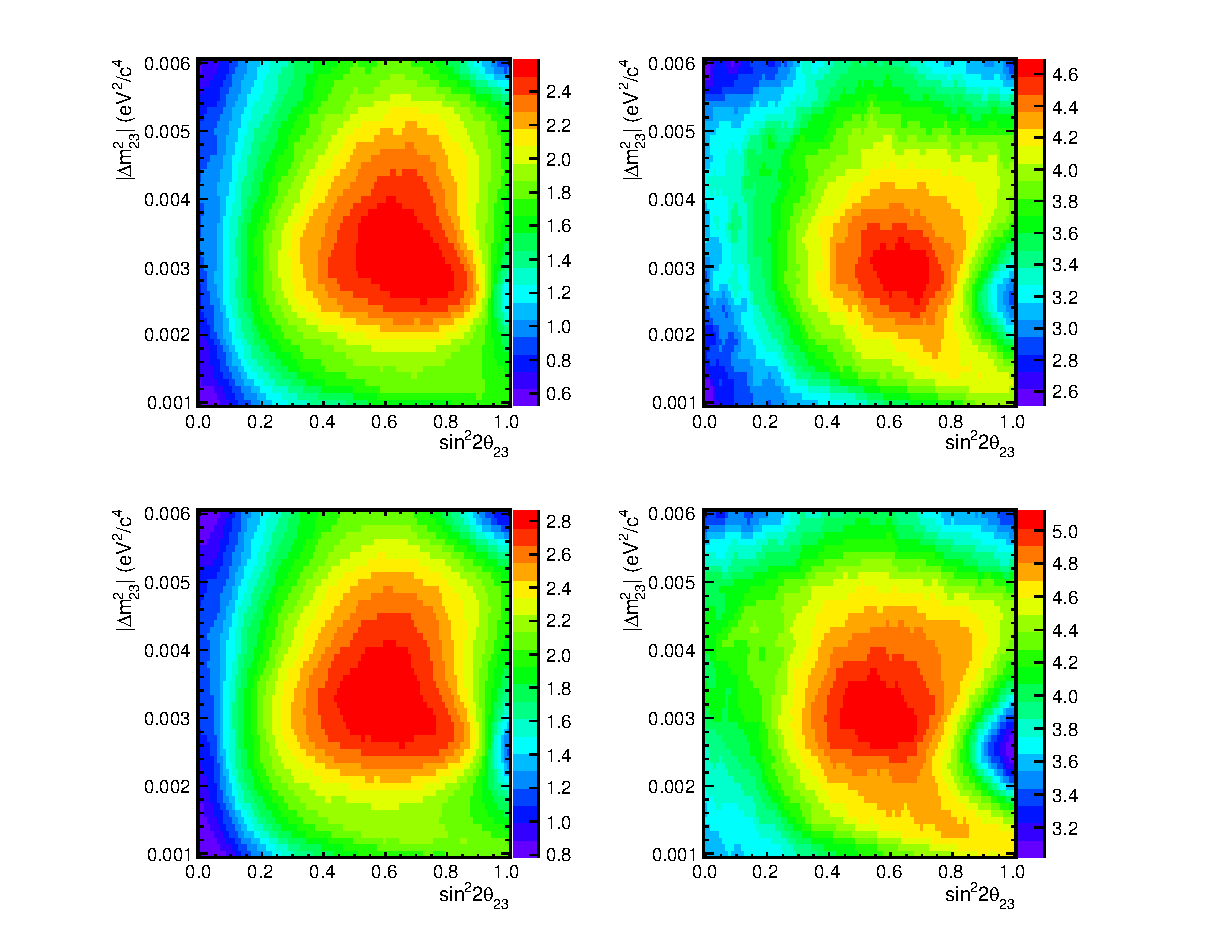
\includegraphics[width=38pc]{./images/fits/feldman_cousins/fc_delta_chisq.eps}
\caption{
  Monte Carlo estimation, 
  according to the Feldman-Cousins method,
  of $\Delta\chi^{2}_{68}$ (left) and $\Delta\chi^{2}_{90}$ (right)
  as functions of $sin^{2}{2\theta_{23}}$ and $\Delta{m^{2}_{23}}$,
  for calculation of the 68\% CL and 90\% CL, respectively, confidence regions
  for the $3.23 \times 10^{19}$-POT T2K $\nu_{\mu}$-disappearance analysis.
  The top row shows $\Delta\chi^{2}$ surfaces calculated using statistical errors
  only whereas the bottom row shows $\Delta\chi^{2}$ surfaces calculated using 
  both statistical and systematic erros.
  We observe that values of $\Delta\chi^{2}$ decrease as one moves closer to the 
  physical boundaries at $sin^{2}{2\theta_{23}}$ = 0 and $sin^{2}{2\theta_{23}}$ = 1 
  and the fit (`search'/`sensitivity') $\Delta{m^{2}_{23}}$ boundaries.
}
\label{fig:fc_delta_chisq}
\end{figure*}

\begin{figure*}[htb]
\center
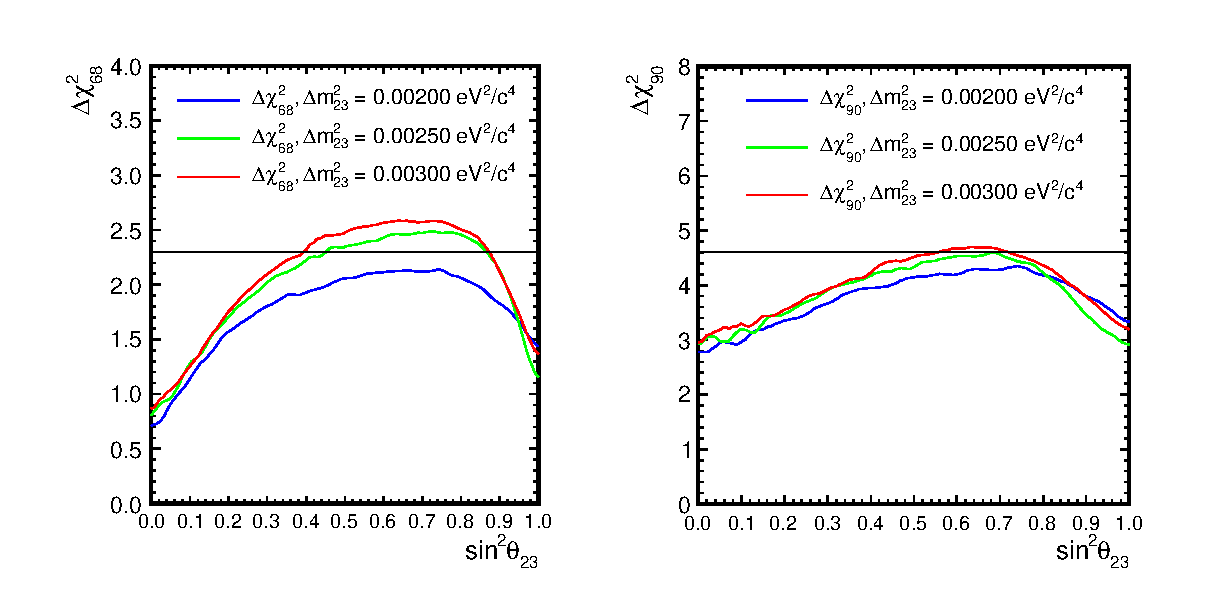
\includegraphics[width=38pc]{./images/fits/feldman_cousins/fc_delta_chisq_stat_vs_sinsq_3dmsq.eps}
\caption{
  Monte Carlo estimation,
  according to the Feldman-Cousins method (statistical errors only),
  of $\Delta\chi^{2}_{68}$ (left) and $\Delta\chi^{2}_{90}$ (right),
  as functions of $sin^{2}{2\theta_{23}}$ for 3 different values of $\Delta{m^{2}_{23}}$ 
  ($2.0 \times 10^{-3} eV^{2}/c^{4}$, 
   $2.5 \times 10^{-3} eV^{2}/c^{4}$ and
   $3.0 \times 10^{-3} eV^{2}/c^{4}$).
  For comparison, the canonical value of $\Delta\chi^{2}$ used in the PDG 
  (see Tab. \ref{table:deltachi2table}) is also shown as a horizontal line.
}
\label{fig:fc_delta_chisq_stat_vs_sinsq_3dmsq}
\end{figure*}

\begin{figure*}[htb]
\center
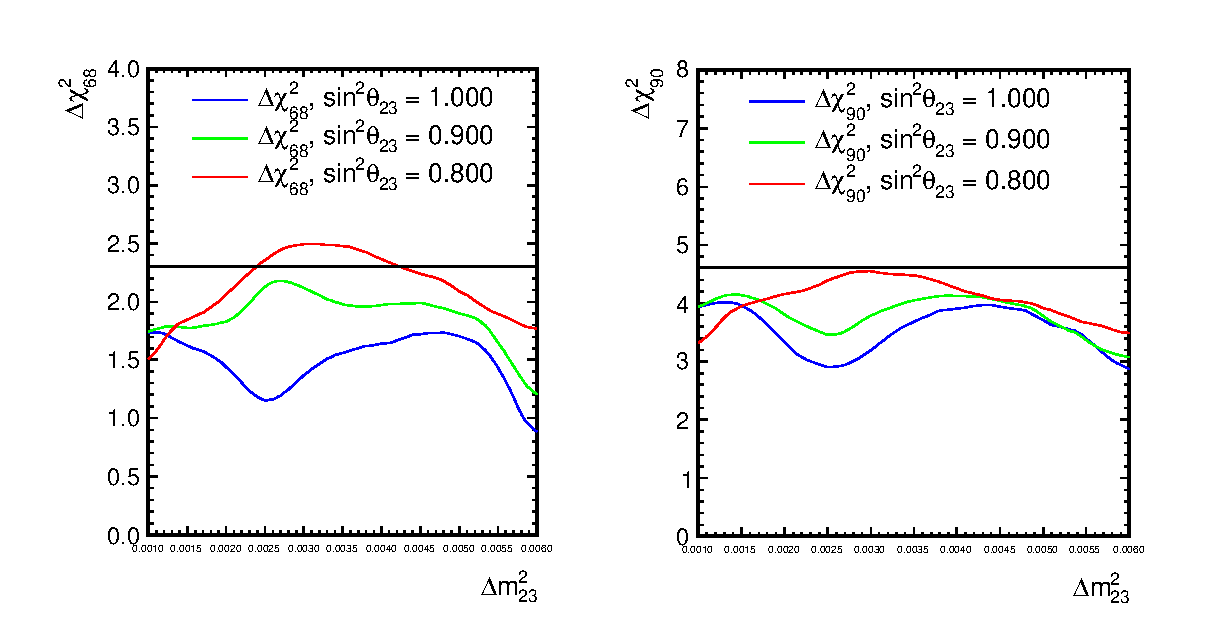
\includegraphics[width=38pc]{./images/fits/feldman_cousins/fc_delta_chisq_stat_vs_dmsq_3sinsq.eps}
\caption{
  Monte Carlo estimation,
  according to the Feldman-Cousins method (statistical errors only),
  of $\Delta\chi^{2}_{68}$ (left) and $\Delta\chi^{2}_{90}$ (right),
  as functions of $\Delta{m^{2}_{23}}$ for 3 different values of $sin^{2}{2\theta_{23}}$ 
  (0.8, 0.9 and 1.0).
  For comparison, the canonical value of $\Delta\chi^{2}$ used in the PDG 
  (see Tab. \ref{table:deltachi2table}) is also shown as a horizontal line.
}
\label{fig:fc_delta_chisq_stat_vs_sinsq_3dmsq}
\end{figure*}


